\documentclass[11pt]{article}
\usepackage[a4paper,margin=1.05in]{geometry}
\usepackage{amsmath,amssymb,amsthm}
\usepackage{booktabs,array,graphicx,xcolor,enumitem}
\usepackage[colorlinks=true,linkcolor=blue!50!black,urlcolor=blue!50!black,citecolor=blue!50!black]{hyperref}
\usepackage{caption}
\captionsetup{font=small,labelfont=bf}
\newcommand{\KWay}{100\,000}
\newcommand{\TotSteps}{491\,665}
\newcommand{\MeanSteps}{4.9166}
\newcommand{\MaxSteps}{6}
\newcommand{\Qsize}{43}
\newcommand{\TotalCases}{323\,103}
\newcommand{\VerSha}{26e8c9f0c3abecda}

\newtheorem{theorem}{Theorem}[section]
\newtheorem{lemma}[theorem]{Lemma}
\newtheorem{proposition}[theorem]{Proposition}
\newtheorem{corollary}[theorem]{Corollary}
\theoremstyle{definition}
\newtheorem{definition}[theorem]{Definition}
\newtheorem{remark}[theorem]{Remark}
\newcommand{\N}{\mathbb{N}}
\newcommand{\dist}{\operatorname{d}}
\newcommand{\RDY}{\mathsf{READY}}

\title{\textbf{Intrinsic Generative Selectors:\\ Finite Control, Arithmetic State, and Observational Realization}\\[4pt]
\large UNNS-U2-001 \,--\, version 1.0 (v001)}
\author{UNNS Research Collective}
\date{8 November 2026}

\begin{document}
\maketitle

\begin{abstract}
\noindent Let $G$ be the graph on the positive integers in which $kN$ is joined to $k(N+1)^2$ for all $k,N\ge1$.
A \emph{selector} chooses one incident edge at every step, from the current integer and a finite control state only,
with no external input. We prove three results. (i)~No deterministic rule that reads only the current integer
can pass through $1,2,3,\dots$ in this order. (ii)~A deterministic rule with $\Qsize$ control states that reads the
current integer by exact arithmetic \emph{can}: it visits $1,2,3,\dots$ in order, reaching each $n+1$ from $n$ in at most six
moves, and the unbounded information needed at each step is carried by the integer itself. (iii)~The doubling
distance is uniformly bounded, $\sup_{n}\dist(n,2n)=5$. The construction in (ii) rests on nine path identities
for $n\to n+1$ whose intermediate states are strictly increasing polynomials in a class parameter, which
makes that parameter recoverable from the current state alone. We also give a precise definition of the selector classes
and show why an unrestricted observation map would make any comparison between them empty.
\end{abstract}

\section{Introduction}\label{sec:intro}
\paragraph{Provenance.} The graph $G$ is the undirected closure of the SELECT-II transformation
$m\mapsto m(N+1)^2/N$ ($N\mid m$) of the UNNS Substrate. Its connectivity and the uniform bound
$\dist(n,n+1)\le6$ are established in the preceding releases~\cite{u1bnd,u1}; the forward-only baseline is
research note U0-001~\cite{u0}. The present release, UNNS-U2-001, leaves all of them unchanged, as it does the
frozen reference collection~\cite{gig,repo}.

\paragraph{Question.} Bounded distance says that every integer can be reached from its predecessor by a short
path. It does not say that a fixed rule can \emph{choose} that path. Can the arithmetic itself determine the next move,
using a fixed rule and no instructions supplied by the desired output sequence?

\paragraph{Results.}
\begin{theorem}[Summary]\label{thm:summary}
\begin{enumerate}[label=(\alph*),nosep]
\item \emph{(U2.0, memoryless obstruction.)} For every function $F:\N_{>0}\to\N_{>0}$ choosing a neighbour of its argument, no orbit
$x_{j+1}=F(x_j)$ contains $1,2,3,\dots$ as a subsequence.
\item \emph{(U2.1, finite-control realization.)} There is a deterministic selector $\Sigma$ with $|Q|=\Qsize$ control states, using
exact integer arithmetic on the current state and no other input, whose trajectory from $x=1$ returns to the ready
control state exactly at $2,3,4,\dots$ in this order, with at most six moves between consecutive ready states.
\item \emph{(Doubling.)} $\dist(n,2n)\le5$ for all $n$, with equality at $n=1$.
\end{enumerate}
\end{theorem}

\section{Graph facts used}\label{sec:facts}
Throughout, $G$ has an edge $\{kN,\,k(N+1)^2\}$ for each pair $k,N\ge1$; a move $+N$ from $x$ requires $N\mid x$ and gives
$x(N+1)^2/N$, and a move $-N$ requires $(N+1)^2\mid x$ and gives $xN/(N+1)^2$. The moves $+N$ and $-N$ are mutually inverse.

\begin{lemma}[Consecutive integers are never adjacent]\label{lem:nonadj}
For $n\ge1$, $\{n,n+1\}$ is not an edge; hence $\dist(n,n+1)\ge2$.
\end{lemma}
\begin{proof} The larger endpoint of an edge is $(N+1)^2/N=N+2+1/N>4$ times the smaller, whereas $(n+1)/n\le2$. \end{proof}

\begin{lemma}[Nine path identities~\cite{u1bnd}]\label{lem:identities}
For every $n\ge1$ there is a path $n=x_0,x_1,\dots,x_\ell=n+1$ with $\ell\le6$ and every step certified, given by one of the nine
parametric families of Appendix~\ref{app:templates} (for $n\in\{1,3\}$, by an explicit path).
\end{lemma}

\begin{lemma}[Doubling]\label{lem:doubling}
$\sup_{n\ge1}\dist(n,2n)=5$.
\end{lemma}
\begin{proof} If $\{x,y\}$ is an edge then so is $\{nx,ny\}$ (multiply $k$ by $n$), so $\dist(na,nb)\le\dist(a,b)$. The path
$1\to4\to18\to81\to8\to2$ (moves $+1,+2,+2,-8,-1$) gives $\dist(1,2)\le5$, hence $\dist(n,2n)\le5$.
For the lower bound, the radius-2 balls are $B_2(1)=\{1,4,16,18,25\}$ and $B_2(2)=\{2,8,9,32,36,48,50,81,100\}$;
they are disjoint, so no path of length $\le4$ joins $1$ and $2$. Thus $\dist(1,2)=5$. \end{proof}

\section{Selector models}\label{sec:models}
\begin{definition}[Selector]\label{def:selector}
A \emph{selector} is a pair $(Q,\Sigma)$ of a finite set $Q$ with a distinguished element $\RDY$ and a function
$\Sigma:\N_{>0}\times Q\to\{+,-\}\times\N_{>0}\times Q$. A configuration $(x,q)$ evolves by $(x,q)\mapsto(x',q')$ where
$\Sigma(x,q)=(\sigma,N,q')$ and $x'$ is the result of the move $\sigma N$ from $x$; $\Sigma$ must return only legal moves. The only
\emph{admissible computation} inside $\Sigma$ is exact arithmetic on the current integer $x$ (addition, multiplication, exact division, comparison, integer
roots, and inversion of strictly increasing integer polynomials); $\Sigma$ receives no target sequence, counter or other external datum.
\end{definition}
\begin{definition}[Realization]\label{def:real}
A trajectory \emph{realizes} $(a_k)_{k\ge1}$ \emph{as raw waypoints} if $a_1,a_2,\dots$ occur among the integers $x_0,x_1,\dots$ at
strictly increasing times $\tau_1<\tau_2<\cdots$. It realizes $(a_k)$ \emph{at completion times} if in addition one may take
$\tau_k$ to be the successive visits of the control state $\RDY$.
\end{definition}
Four classes are compared.
\begin{center}\small
\begin{tabular}{@{}lll@{}}\toprule
class & definition & extra input\\\midrule
$\mathcal S_0$ state-only & $|Q|=1$ (a function of $x$) & none\\
$\mathcal S_1$ finite control & $|Q|<\infty$, arithmetic on $x$ as above & none\\
$\mathcal S_2$ unbounded memory & $Q$ replaced by a counter or tape & none\\
$\mathcal S_3$ external targets & $\Sigma$ may read the target sequence & the sequence\\\bottomrule
\end{tabular}
\end{center}
Here $\mathcal S_0\subseteq\mathcal S_1\subseteq\mathcal S_2\subseteq\mathcal S_3$ by definition. Which inclusions are strict for the identity sequence is the content of
Sections~\ref{sec:obstruction}--\ref{sec:classes}.

\section{The memoryless obstruction}\label{sec:obstruction}
\begin{theorem}[U2.0]\label{thm:u20}
No $\mathcal S_0$ selector, i.e.\ no function $F$ with $F(x)$ a neighbour of $x$, has an orbit containing $1,2,3,\dots$ as raw waypoints.
\end{theorem}
\begin{proof} Suppose the orbit $(x_j)$ does. If some value is revisited, $x_i=x_j$ with $i<j$, determinism makes the orbit eventually periodic, so it takes only
finitely many values and cannot contain all positive integers. Hence the orbit is injective, and each integer $m$ occurs exactly once, at time $\tau_m$, with
$\tau_1<\tau_2<\cdots$. Every $x_j$ is a positive integer $m$, so $j=\tau_m$. If $\tau_{m+1}>\tau_m+1$, the state $x_j$ at some $j$ with $\tau_m<j<\tau_{m+1}$ would be an integer $m'$ with $\tau_{m'}=j$, contradicting the monotonicity of
$\tau$; and the same argument excludes states before $\tau_1$. So $\tau_{m+1}=\tau_m+1$ and $x_{j+1}=x_j+1$, i.e.\ $\{m,m+1\}$ is an edge, contradicting
Lemma~\ref{lem:nonadj}. \end{proof}
\begin{remark} Only Lemma~\ref{lem:nonadj} is used; the bound $\dist\le6$ plays no role. The obstruction holds for any graph on $\N_{>0}$ in which no two consecutive integers are adjacent.\end{remark}

\section{Finite-control successor generation}\label{sec:finite}
\subsection{The selector}
For each class $c\in\{A,\dots,I\}$ let $n=Mt+r$ ($t\ge t_0$) be its residue form, with moves $\sigma_1N_1,\dots,\sigma_\ell N_\ell$ whose labels $N_i=N_i(t)$ are given in Appendix~\ref{app:templates}, and let
$s_0(t)=n,\ s_1(t),\dots,s_\ell(t)=n+1$ be the successive states. The control set is
\begin{multline*} Q=\{\RDY\}\ \cup\ \{(c,i):c\in\{A,\dots,I\},\,1\le i<\ell_c\}\\ \cup\ \{(S_1,i)\}_{i=1}^4\cup\{(S_3,1)\}, \end{multline*}
of size $\Qsize$. The selector is:
\begin{itemize}[nosep]
\item $\Sigma(1,\RDY)$ and $\Sigma(3,\RDY)$ begin the fixed special paths $1\to4\to18\to81\to8\to2$ and $3\to16\to4$ (finitely many table entries).
\item $\Sigma(x,\RDY)$ for other $x$: let $c$ be the class of the residue of $x$ ($\bmod 24$), let $t$ be the unique solution of $s_0(t)=x$, and play move $\sigma_1N_1(t)$ with new control $(c,1)$ (or $\RDY$ if $\ell_c=1$).
\item $\Sigma(x,(c,i))$: let $t$ be the unique solution of $s_i(t)=x$ with $t\ge t_0$, play move $\sigma_{i+1}N_{i+1}(t)$, and change control to $(c,i+1)$, or to $\RDY$ if $i+1=\ell_c$.
\end{itemize}

\begin{lemma}[Recoverability]\label{lem:recover}
For each class $c$ and each $0\le i\le\ell_c$ the state $s_i(t)$ is a strictly increasing polynomial on $t\ge t_0$ with rational coefficients, taking integer values.
Hence $t$ is determined by $(c,i,x)$ and is computed by exact arithmetic (for example binary search on a monotone integer polynomial).
\end{lemma}
\begin{proof} The states $s_i(t)$ are listed in Appendix~\ref{app:templates} in factored form; each is a product of positive powers of linear forms in $t$ with positive coefficients
on $t\ge t_0$, hence strictly increasing. Symbolic verification: check W3 of Table~\ref{tab:status}. \end{proof}
\begin{remark}[Example] In class $A$ ($n=4t+1$): $4t+1\to4(2t+1)^2\to8t\to8(t+1)^2\to2(2t+1)$. At the third state $t=x/8$, at the fourth $t=\sqrt{x/8}-1$.\end{remark}

\begin{theorem}[U2.1]\label{thm:u21}
The selector $\Sigma$ is a legal $\mathcal S_1$ selector. From $(1,\RDY)$ its trajectory returns to $\RDY$ exactly at $2,3,4,\dots$ in order; each return takes between $2$ and $6$ moves.
\end{theorem}
\begin{proof} By Lemma~\ref{lem:recover}, $\Sigma$ is a well-defined function of $(x,q)$. For $x=n\ge1$ in $\RDY$ with $n\notin\{1,3\}$, the parameter $t$ is determined and the states visited are
$s_1(t),\dots,s_\ell(t)=n+1$ because the identities of Lemma~\ref{lem:identities} are exactly these compositions; every move is legal by the certificates of~\cite{u1bnd}.
At $n+1$ control returns to $\RDY$. The special paths end at $2$ and $4$. Induction on $n$ completes the proof. \end{proof}
\begin{remark}[Consistency with U2.0]
Projecting onto $x$ alone, the same integer occurs under different controls with different moves (the verifier exhibits one), so the trajectory is not the orbit of any $\mathcal S_0$ selector. The control component is
only a finite step counter, and the template index fixed by the residue of $n$; no counter grows with $n$.
\end{remark}
\begin{corollary}[Cost]\label{cor:cost}
After $K$ waypoints, at most $6K$ moves have been made.
\end{corollary}
\begin{figure}[ht]\centering
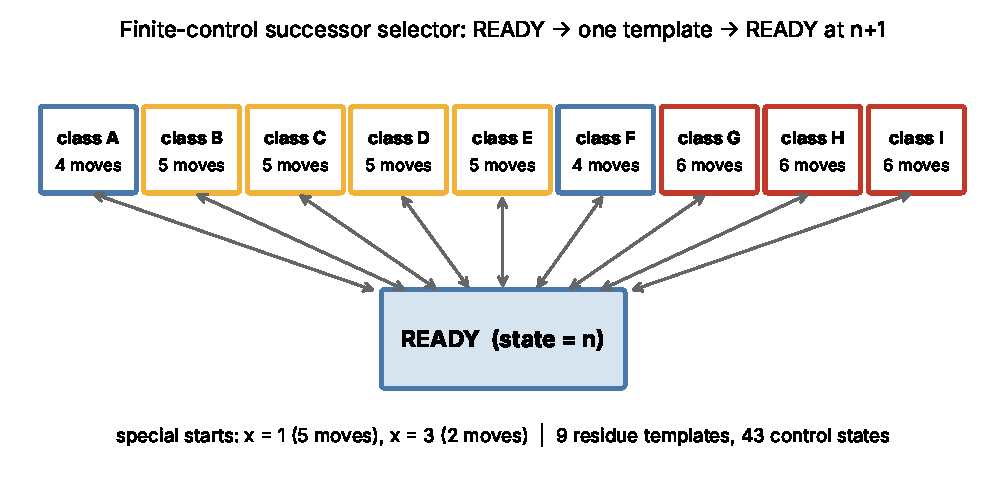
\includegraphics[width=.86\textwidth]{figures/fig1_control_automaton.pdf}
\caption{Control structure of $\Sigma$. From $\RDY$ a residue class selects one of nine templates; the template runs to completion and returns to $\RDY$ at $n+1$.}
\end{figure}
\begin{figure}[ht]\centering
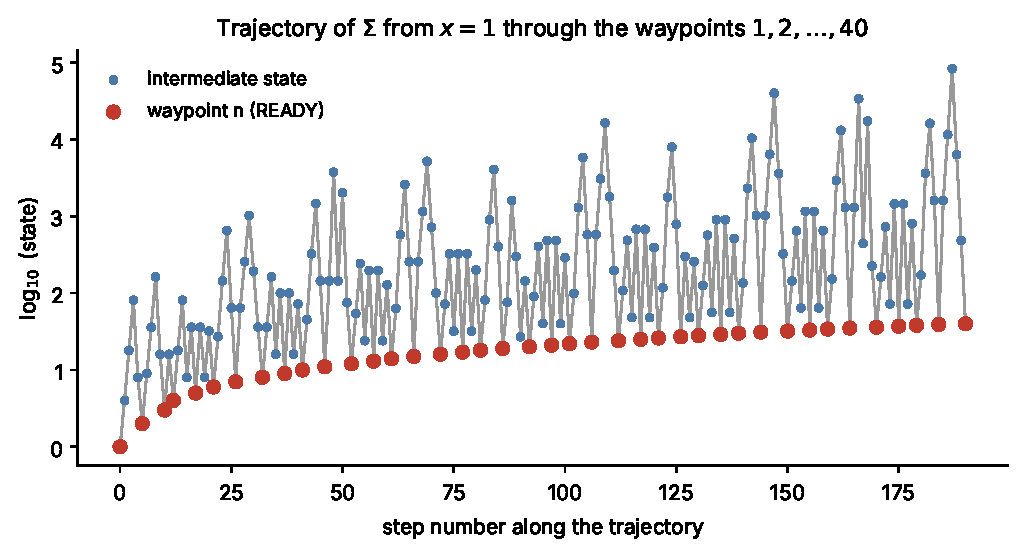
\includegraphics[width=.86\textwidth]{figures/fig2_trajectory.pdf}
\caption{The trajectory of $\Sigma$ from $x=1$ through the first forty waypoints on a logarithmic scale.}
\end{figure}

\subsection{Computational validation}
The long-run test below is a validation of the formal argument, not a substitute for it. Over $\KWay$ successive waypoints the selector made $\TotSteps$ moves, mean $\MeanSteps$ per waypoint, maximum $\MaxSteps$; every move was checked against the edge definition.
\begin{center}\begin{tabular}{rr}\toprule steps to next waypoint & count\\\midrule
2 & 1 \\
4 & 29\,165 \\
5 & 50\,001 \\
6 & 20\,833 \\
\bottomrule\end{tabular}
\end{center}

\section{What the classes can and cannot distinguish}\label{sec:classes}
\begin{proposition}[Separation for the identity sequence]\label{prop:sep}
The identity sequence is realized as raw waypoints by $\mathcal S_1$ (Theorem~\ref{thm:u21}) and not by $\mathcal S_0$ (Theorem~\ref{thm:u20}). Therefore $\mathcal S_0\subsetneq\mathcal S_1$ at the level of realizable sequences.
\end{proposition}
\begin{proposition}[Unrestricted observation trivializes the comparison]\label{prop:obs}
Let $F(x)=4x$ (the move $+1$, legal at every $x$). Its orbit from $x=1$ is $4^j$. For any computable sequence $(a_k)$ the observation $o(x)=a_{\log_4x}$ (defined on powers of $4$) turns this state-only selector into one whose observations realize $(a_k)$.
\end{proposition}
Consequently an observation map cannot be an arbitrary computable function. In this release a realization is always read directly from the integer states (raw waypoints) or from visits to $\RDY$; any further restriction on observation, such as bounded-memory or length-preserving read-outs, is an open design choice and is not needed for the results above.

\section{A criterion for native generation}\label{sec:native}
\begin{definition}[Native realization]\label{def:native}
A selector $(Q,\Sigma)$ \emph{natively realizes} $(a_k)$ if (1) $\Sigma$ is one fixed finite object, independent of $k$; (2) it receives no external input; (3) $(a_k)$ occurs as raw waypoints or at $\RDY$ completion times; (4) the only unbounded quantity it uses at any step is the current integer.
\end{definition}
Theorem~\ref{thm:u21} says that the identity sequence is natively realized in $\mathcal S_1$. What was supplied is finite: nine templates and two special paths. What was not supplied is the sequence. In this sense the selector generates $1,2,3,\ldots$ and does not merely traverse it.
\paragraph{Limits of the claim.} The result concerns a sequence whose consecutive terms are uniformly close in $G$; the selector encodes the one finite fact ``how to reach $n+1$ from $n$ in at most six moves''. The criterion does not yet say which other sequences admit such a selector.

\section{Status and open questions}\label{sec:status}
\begin{table}[ht]\centering\small
\begin{tabular}{@{}p{0.25\textwidth}p{0.18\textwidth}p{0.45\textwidth}@{}}\toprule
statement & status & basis\\\midrule
U2.0 obstruction & proved & elementary argument; ingredient checked to $n\le20000$ (W7)\\
Recoverability & proved & polynomial monotonicity; symbolic check, 55 states (W3)\\
U2.1 realization & proved, computer-supported & uses certified identities of~\cite{u1bnd}; long-run validation (W5, W6)\\
Doubling $=5$ & proved & Lemma~\ref{lem:doubling}; replay to $2\times10^5$ and two-engine ball check (W1, W2)\\
Formal proof-assistant certification & not done & --\\
Literature originality review & not done & --\\\bottomrule
\end{tabular}
\caption{Status of the results. All verifier checks passed (\TotalCases{} cases; verifier hash prefix \texttt{\VerSha}).}\label{tab:status}
\end{table}
\paragraph{Open questions.}
\begin{enumerate}[nosep]
\item Which sequences other than $1,2,3,\ldots$ are natively realized in $\mathcal S_1$: squares, primes, Fibonacci numbers? For squares one needs a uniform bound on $\dist(n^2,(n+1)^2)$ and a decodable family of path identities; for primes the unbounded search seems to need more than finite control.
\item Is every sequence with uniformly bounded waypoint distance and a recoverable path family realizable in $\mathcal S_1$? What replaces recoverability when the intermediate states are not monotone in a single parameter?
\item What is the right restriction on observation maps so that comparisons between selector classes remain informative?
\end{enumerate}

\appendix
\section{The nine templates}\label{app:templates}
Each line lists the states and the moves (labels over arrows) of one class, in factored form, from the symbolic composition of the certified identities.
{\small\paragraph{Class A.} $n=4t+1$, $t\ge 1$:
\begin{gather*}
4 t + 1 \xrightarrow{+\left(4 t + 1\right)} 4 \left(2 t + 1\right)^{2} \xrightarrow{-2 t} 8 t \\
8 t \xrightarrow{+t} 8 \left(t + 1\right)^{2} \xrightarrow{-\left(2 t + 1\right)} 2 \left(2 t + 1\right)
\end{gather*}
\paragraph{Class B.} $n=8t$, $t\ge 1$:
\begin{gather*}
8 t \xrightarrow{+2} 36 t \xrightarrow{+2} 162 t \\
162 t \xrightarrow{-8} 16 t \xrightarrow{+4 t} 4 \left(4 t + 1\right)^{2} \\
4 \left(4 t + 1\right)^{2} \xrightarrow{-\left(8 t + 1\right)} 8 t + 1
\end{gather*}
\paragraph{Class C.} $n=8t+2$, $t\ge 0$:
\begin{gather*}
2 \left(4 t + 1\right) \xrightarrow{+2} 9 \left(4 t + 1\right) \xrightarrow{+\left(4 t + 1\right)} 36 \left(2 t + 1\right)^{2} \\
36 \left(2 t + 1\right)^{2} \xrightarrow{+2} 162 \left(2 t + 1\right)^{2} \xrightarrow{-8} 16 \left(2 t + 1\right)^{2} \\
16 \left(2 t + 1\right)^{2} \xrightarrow{-\left(8 t + 3\right)} 8 t + 3
\end{gather*}
\paragraph{Class D.} $n=8t+4$, $t\ge 0$:
\begin{gather*}
4 \left(2 t + 1\right) \xrightarrow{+2} 18 \left(2 t + 1\right) \xrightarrow{+2} 81 \left(2 t + 1\right) \\
81 \left(2 t + 1\right) \xrightarrow{-8} 8 \left(2 t + 1\right) \xrightarrow{+2 \left(2 t + 1\right)} 4 \left(4 t + 3\right)^{2} \\
4 \left(4 t + 3\right)^{2} \xrightarrow{-\left(8 t + 5\right)} 8 t + 5
\end{gather*}
\paragraph{Class E.} $n=8t+6$, $t\ge 0$:
\begin{gather*}
2 \left(4 t + 3\right) \xrightarrow{+2} 9 \left(4 t + 3\right) \xrightarrow{+\left(4 t + 3\right)} 144 \left(t + 1\right)^{2} \\
144 \left(t + 1\right)^{2} \xrightarrow{+2} 648 \left(t + 1\right)^{2} \xrightarrow{-8} 64 \left(t + 1\right)^{2} \\
64 \left(t + 1\right)^{2} \xrightarrow{-\left(8 t + 7\right)} 8 t + 7
\end{gather*}
\paragraph{Class F.} $n=24t+3$, $t\ge 1$:
\begin{gather*}
3 \left(8 t + 1\right) \xrightarrow{+\left(8 t + 1\right)} 12 \left(4 t + 1\right)^{2} \xrightarrow{-4 t} 48 t \\
48 t \xrightarrow{+3 t} 16 \left(3 t + 1\right)^{2} \xrightarrow{-\left(6 t + 1\right)} 4 \left(6 t + 1\right)
\end{gather*}
\paragraph{Class G.} $n=8t+7$, $t\ge 0$:
\begin{gather*}
8 t + 7 \xrightarrow{+\left(8 t + 7\right)} 64 \left(t + 1\right)^{2} \xrightarrow{+\left(t + 1\right)} 64 \left(t + 1\right) \left(t + 2\right)^{2} \\
64 \left(t + 1\right) \left(t + 2\right)^{2} \xrightarrow{+\left(t + 1\right)} 64 \left(t + 2\right)^{4} \xrightarrow{-\left(2 t + 3\right)} 16 \left(t + 2\right)^{2} \left(2 t + 3\right) \\
16 \left(t + 2\right)^{2} \left(2 t + 3\right) \xrightarrow{-\left(2 t + 3\right)} 4 \left(2 t + 3\right)^{2} \xrightarrow{-2 \left(t + 1\right)} 8 \left(t + 1\right)
\end{gather*}
\paragraph{Class H.} $n=24t+11$, $t\ge 0$:
\begin{gather*}
24 t + 11 \xrightarrow{+\left(24 t + 11\right)} 144 \left(2 t + 1\right)^{2} \xrightarrow{+24} 3750 \left(2 t + 1\right)^{2} \\
3750 \left(2 t + 1\right)^{2} \xrightarrow{-2 \left(25 t + 12\right)} 12 \left(25 t + 12\right) \xrightarrow{+\left(25 t + 12\right)} 12 \left(25 t + 13\right)^{2} \\
12 \left(25 t + 13\right)^{2} \xrightarrow{-25 \left(2 t + 1\right)} 75 \left(2 t + 1\right) \xrightarrow{-4} 12 \left(2 t + 1\right)
\end{gather*}
\paragraph{Class I.} $n=24t+19$, $t\ge 0$:
\begin{gather*}
24 t + 19 \xrightarrow{+1} 4 \left(24 t + 19\right) \xrightarrow{+\left(24 t + 19\right)} 64 \left(6 t + 5\right)^{2} \\
64 \left(6 t + 5\right)^{2} \xrightarrow{-3} 12 \left(6 t + 5\right)^{2} \xrightarrow{-3 \left(4 t + 3\right)} 9 \left(4 t + 3\right) \\
9 \left(4 t + 3\right) \xrightarrow{+\left(4 t + 3\right)} 144 \left(t + 1\right)^{2} \xrightarrow{-\left(6 t + 5\right)} 4 \left(6 t + 5\right)
\end{gather*}
}

\section{Reproducibility}\label{app:repro}
From the directory \texttt{code/}: \texttt{python3 verify\_u2\_001.py --out ../reports/u2\_001\_verification\_report.json --data ../data}\linebreak (about three minutes). The files \texttt{u1\_bnd\_lib.py} (unchanged from the U1-BND release) and
\texttt{u2\_selector.py} define the graph primitives and $\Sigma$. Use \texttt{python3} without the \texttt{-I} flag, from \texttt{code/}. The verifier does not re-run the heavy checks of the earlier releases (recorded as NOT\_RERUN with hashes in the README).

\begin{thebibliography}{9}
\bibitem{u0} UNNS Research Collective, \emph{UNNS-U0: Arithmetic reachability and orbit admissibility}, research note U0-001, 8 November 2026 (local release; not part of the frozen repository).
\bibitem{u1} UNNS Research Collective, \emph{UNNS-U1: Reversible arithmetic connectivity}, research note, 8 November 2026 (provisional baseline; local release).
\bibitem{u1bnd} UNNS Research Collective, \emph{Bounded Successor Distance in the Reversible Square-Multiplication Graph}, UNNS-U1-BND version 1.0 (v001), 8 November 2026 (local release).
\bibitem{gig} UNNS Research Collective, \emph{UNNS Generative Information Geometry collection}, frozen release, repository \texttt{ukbbi/UNNS}, commit \texttt{a115e4bc6b8ee734e6146b3b17a6b121e65d31c3}:
\url{https://github.com/ukbbi/UNNS/tree/a115e4bc6b8ee734e6146b3b17a6b121e65d31c3/projects/UNNS_Generative_Information_Geometry}.
\bibitem{repo} UNNS project repository, pinned at the same commit:
\url{https://github.com/ukbbi/UNNS/tree/a115e4bc6b8ee734e6146b3b17a6b121e65d31c3}.
\end{thebibliography}
\end{document}
